% !TEX root = ../../../main.tex
% 来源：高中物理甲种本·第一册（力学）
% 章节：直线运动 / 变速直线运动~~平均速度~~即时速度
% 原始文件：2.tex，行 672-689
% 类型：tikz
% ---
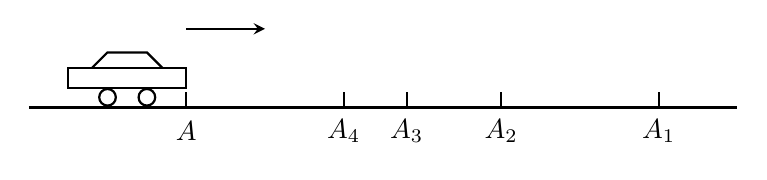
\begin{tikzpicture}[>=stealth,  thick, scale=1]

\draw (0,0)--(9,0);

\foreach \x in {2,4,4.8,6, 8}
{
   \draw (\x,0)--(\x, .2);
}
\draw[->] (2,1)--(3,1);
\node at (2,-.3){$A$};\node at (8,-.3){$A_1$};\node at (6,-.3){$A_2$};\node at (4.8,-.3){$A_3$};\node at (4,-.3){$A_4$};

\draw (.5,.25) rectangle (2,.5);

\draw  (.8,.5)--(1,.7)--(1.5,.7)--(1.7,.5);
\draw  (1,.13) circle [radius=3pt]; 
\draw  (1.5,.13) circle [radius=3pt]; 

\end{tikzpicture}
